%! TEX root = **/000-main.tex
% vim: spell spelllang=en:

\section{Visão Geral}%
    \subsection{Tema/Contexto/gênero}%
    \label{sec:contexto}
    A tematica principal do jogo será a de frutos do mar, sendo usados tanto elementos biologia/vida marinha quanto de seus usos culinarios.
    Para trazer essa ideia a vida sera usado o gênero de platformer com elementos de ação, sendo um tradicional "corre e atira".\\

    \subsection{Mecânicas Central}%
    \label{sec:mecanica}
    Como mencionado em \Cref{sec:contexto} o jogo será um "corre e atira" logo as principais mecânicas serão as de movimentação e combate.\\

        \subsubsection{Movimentação}\label{sec:mecanica:movimentação}

        \begin{itemize}
        \item andar para a esquerda
        \item andar para a direita
        \item saltar
        \item mecânica de dash
        \end{itemize}

        \subsubsection{Combate}\label{sec:mecanica:combate}
        Já no combate, haverá 2 ataques disponiveis para o jogador:

        \begin{itemize}
          \item Um ataque a curta distância usando a pinça, o ataque percorrera uma curta faixa logo a frente do protagonista, dando dano em tudo naquela area.
          \item Um ataque a distância, sendo um disparo de agua emitido da pinça do personagem, percorre uma distância muito maior que o ataque melee, porém causando menos dano, e que depende de munição (agua) para ser ultilizado.
        \end{itemize}

    \subsection{Controles}%
    Para o gameplay serão usados as teclas com a seguinte disposição:
    \begin{figure}[H]
        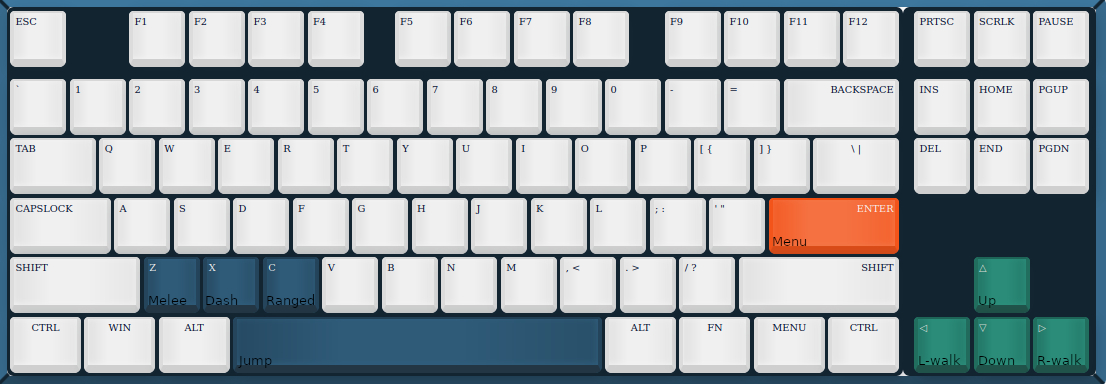
\includegraphics[width=15cm]{keyboard}
    \centering
    \end{figure}

    \subsection{Plataformas Alvo}%
    Inicialmente PC:
        \begin{itemize}
            \item Windowns
            \item Linux
        \end{itemize}
    Porém com possivel expanção para consoles em caso de sucesso.
    \subsection{Público Alvo}%
        Publico jovem, gen z, que gostam do tipo de humor nonsense, afinal o protagonista é um camarão solitário em busca de amor, mas que não abrem mão da experiencia de jogar um bom platformer.

    \subsection{Escopo do Projeto}%
    \subsubsection{Tempo de desenvolvimento}
        De 3 a 4 meses.

    \subsubsection{O que será implementado}
        \begin{itemize}
            \item Todo o core da mecânica básica.
            \item Pelo menos 3 fases (ou mundos)
            \item Geração dinâmica de inimigos, cada vez que se joga uma fase a experiencia será unica.
        \end{itemize}
    \subsubsection{O que pode ser implementado}
        \begin{itemize}
            \item sistema de skins e/ou equipamentos, apenas para a estética, sem alteração do gameplay.
            \item sistema de score/achievements.
        \end{itemize}

    \subsubsection{Equipe}
        \begin{itemize}
            \item Silmar Pereira da Silva Junior: Programação, Design, DevOps;
            \item João Paulo Garcia Martinelli de Oliveira: programação e arquitetura dos leveis;
            \item Lucas Gabriel Mendes Miranda: design;
            \item Flavio Ippolito Vasini Design;
            \item Leonardo Vinícius de Almeida: programador;
        \end{itemize}

    \subsection{Influências}%
        \subsubsection{Megaman:}
        \label{sec:influencias:megaman}
            \begin{figure}[H]
                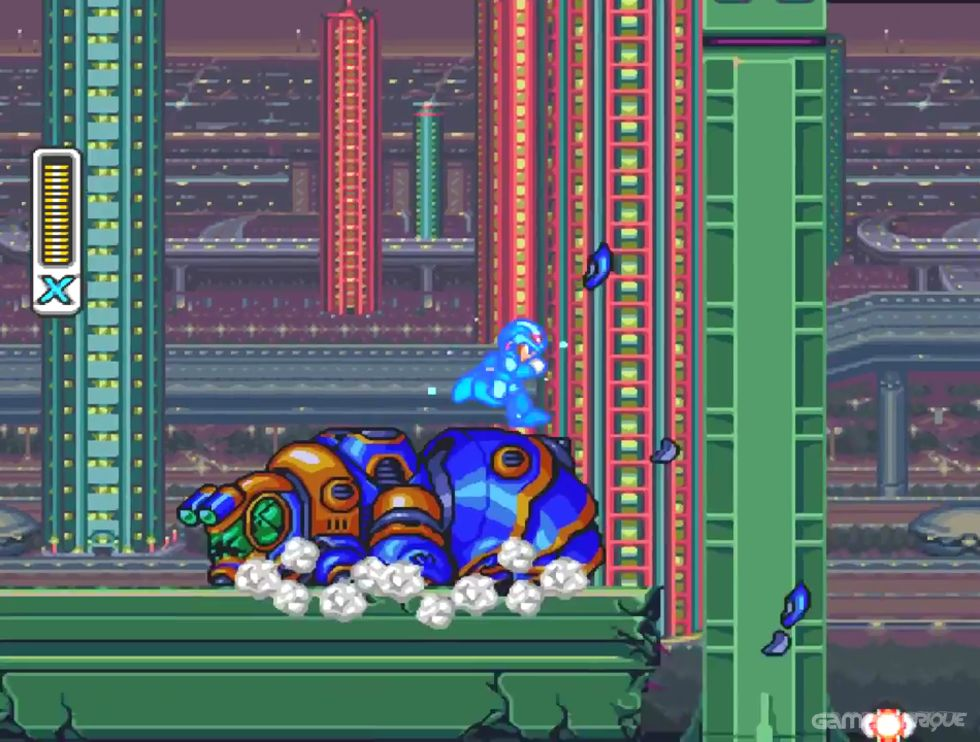
\includegraphics[width=8cm]{Megaman}
            \centering
            \end{figure}

        Megaman é a principal referência quanto ao gameplay, bastante da mecânica é inspirada no jogo, como mencionado na \Cref{sec:mecanica}, correr, pular e atirar são as principais atividades desenpenhadas por X (protagonista do Megaman X) e pelo camarão. Ademais, em subsequentes jogos da franquia, houve a adição de mais um personagem jogável, o Zero, que usa sua espada para causar ataques de curta distância, dos quais o golpe melee do protagonista é baseado.\\
        Além das mecânicas de movimentação e combate, outro elemento que Megaman servirá de inspiração será no level design, com fases bem projetadas para oferecer desafios ao jogador e um boss no final.\\

        \subsubsection{Cuphead:}
            \begin{figure}[H]
                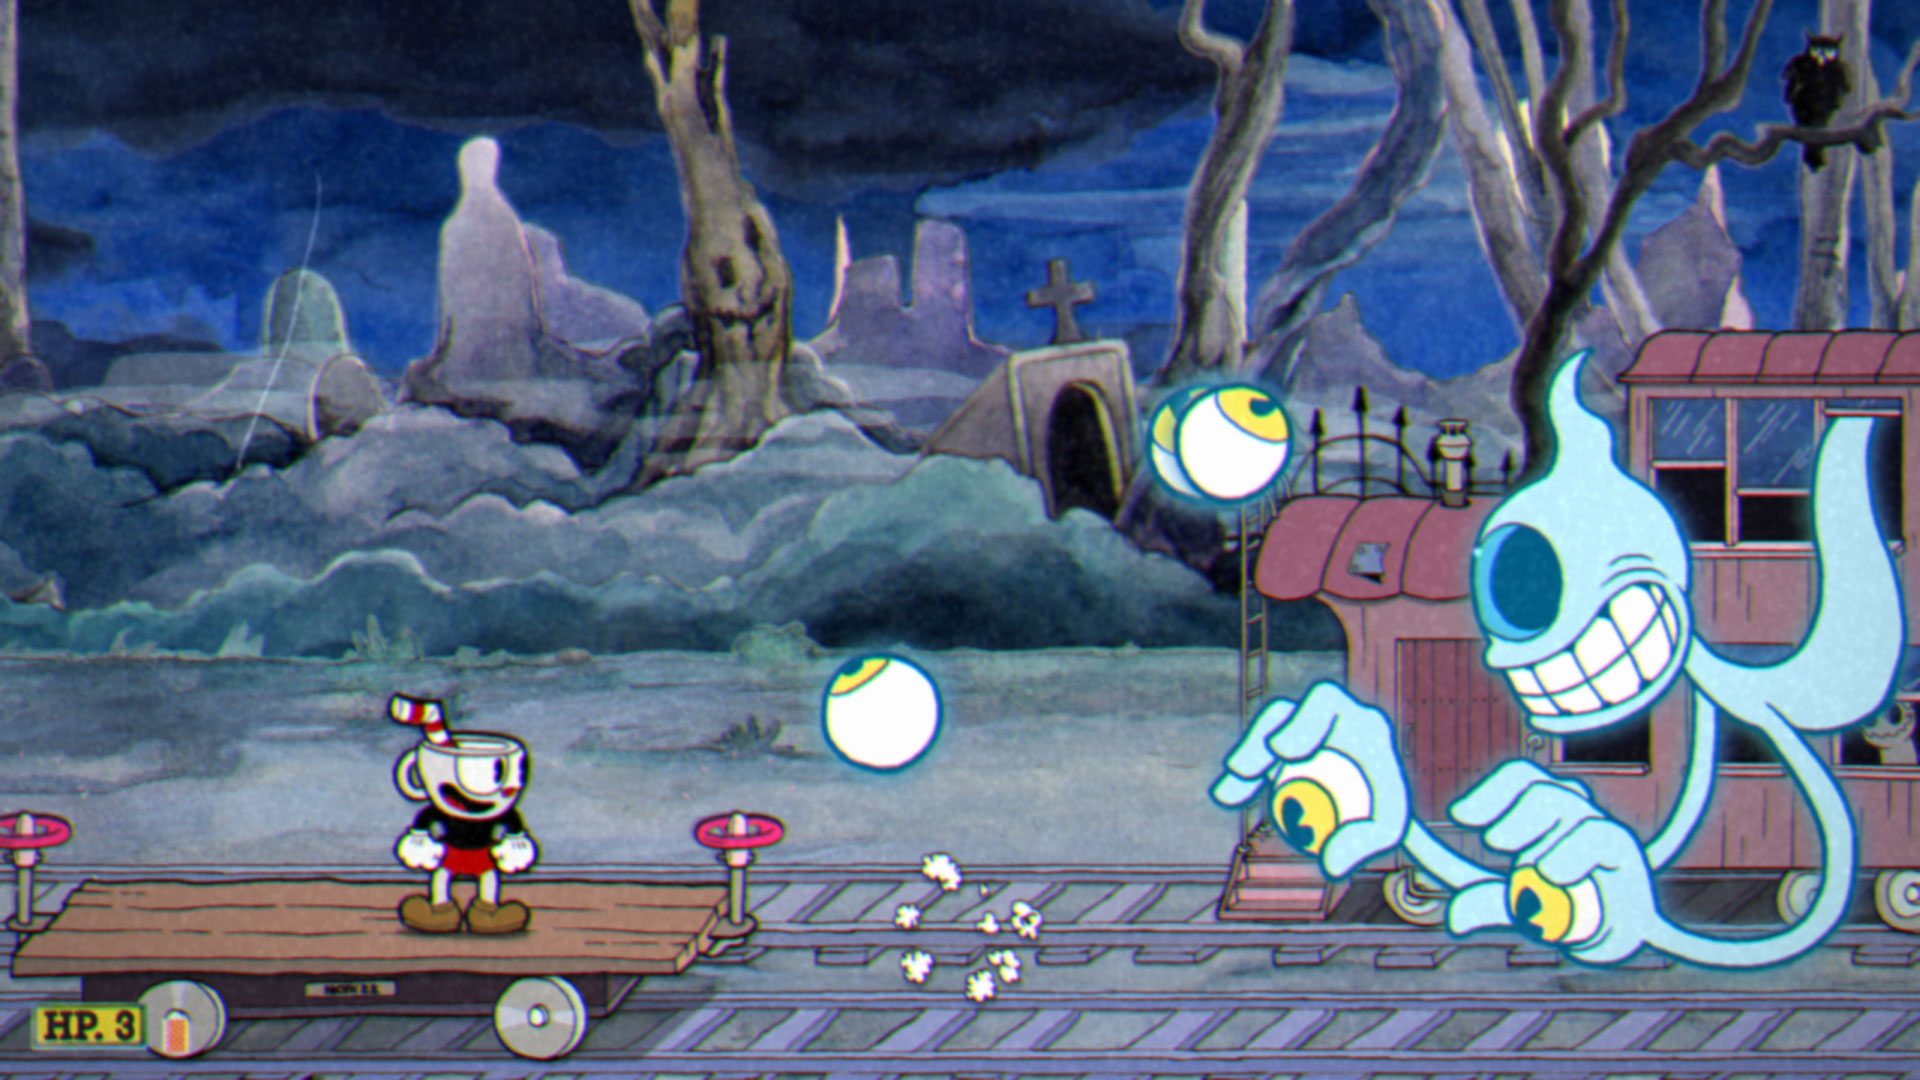
\includegraphics[width=10cm]{Cuphead}
            \centering
            \end{figure}

            Cuphead, será a inspiração quanto ao design de personagens, cenários, inimigos e tudo relacionado ao artistico do projeto, sendo bem colorido e cartunesco.\\
            Também vale resaltar que varias das mecânicas mencionadas em \Cref{sec:influencias:megaman} são compartilhadas com Cuphead e também serão consideradas como formas de inspiração, apesar das influências usadas de Cuphead serem mais voltadas ao artístico e nem tanto ao gameplay.\\

        \subsubsection{Biologia:}
            \begin{figure}[H]
                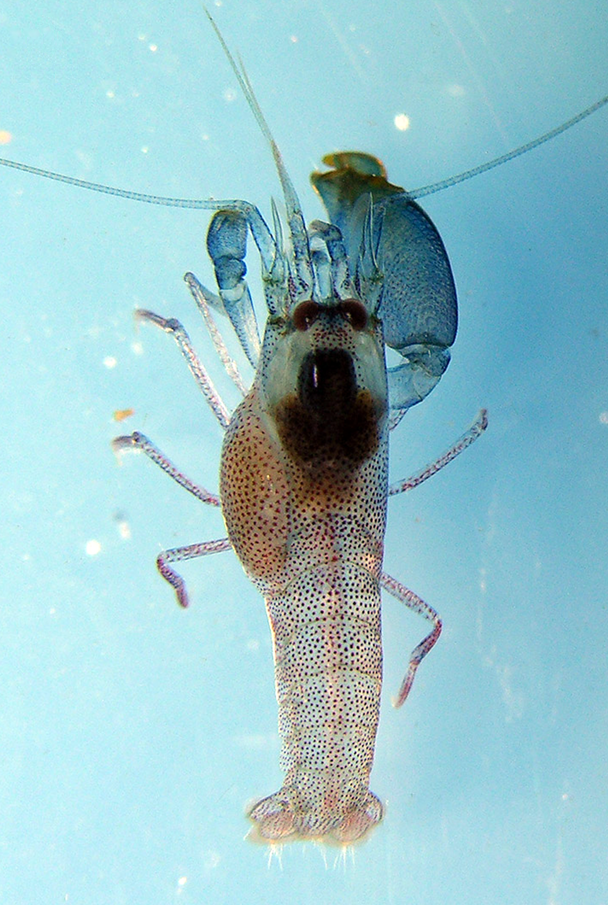
\includegraphics[width=5cm]{PistolShrimp}
            \centering
            \end{figure}

            A especie de camarão \textit{Synalpheus fritzmuelleri} mais conhecida como camarão-pistola é a grande inspiração para o protagonista do jogo, essa especie possui uma pinça direita peculiar, que é capaz de ao fechar e precionar a agua dentro dela produz uma onda de choque que se move pela agua tão forte que é capaz de nocautear suas presas.
 
        \subsubsection{CupNoodles de frutos do mar:}
            \begin{figure}[H]
                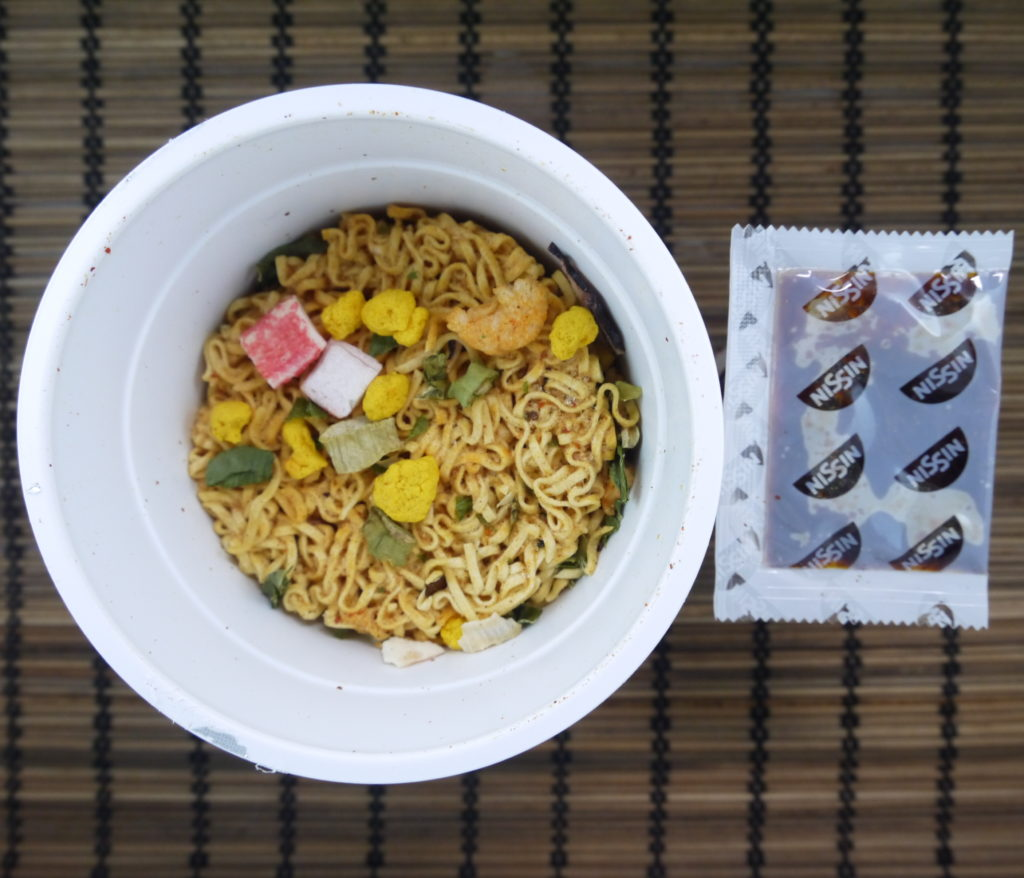
\includegraphics[width=10cm]{CupNoodles}
            \centering
            \end{figure}
            
            Todo CupNoodles tem acompanhamentos que vem junto do macarrão e no de frutos do mar não é diferente, mas já tentou achar um camarão nele, garantimos que há no maximo 1 por pacote, ele está lá, sozinho, apenas esperando que se ponha agua quente, espere 3 minutinhos e acabe com sua solidão.

        \subsubsection{O sexto sentido - M. Night Shyamalan}
            \begin{figure}[H]
                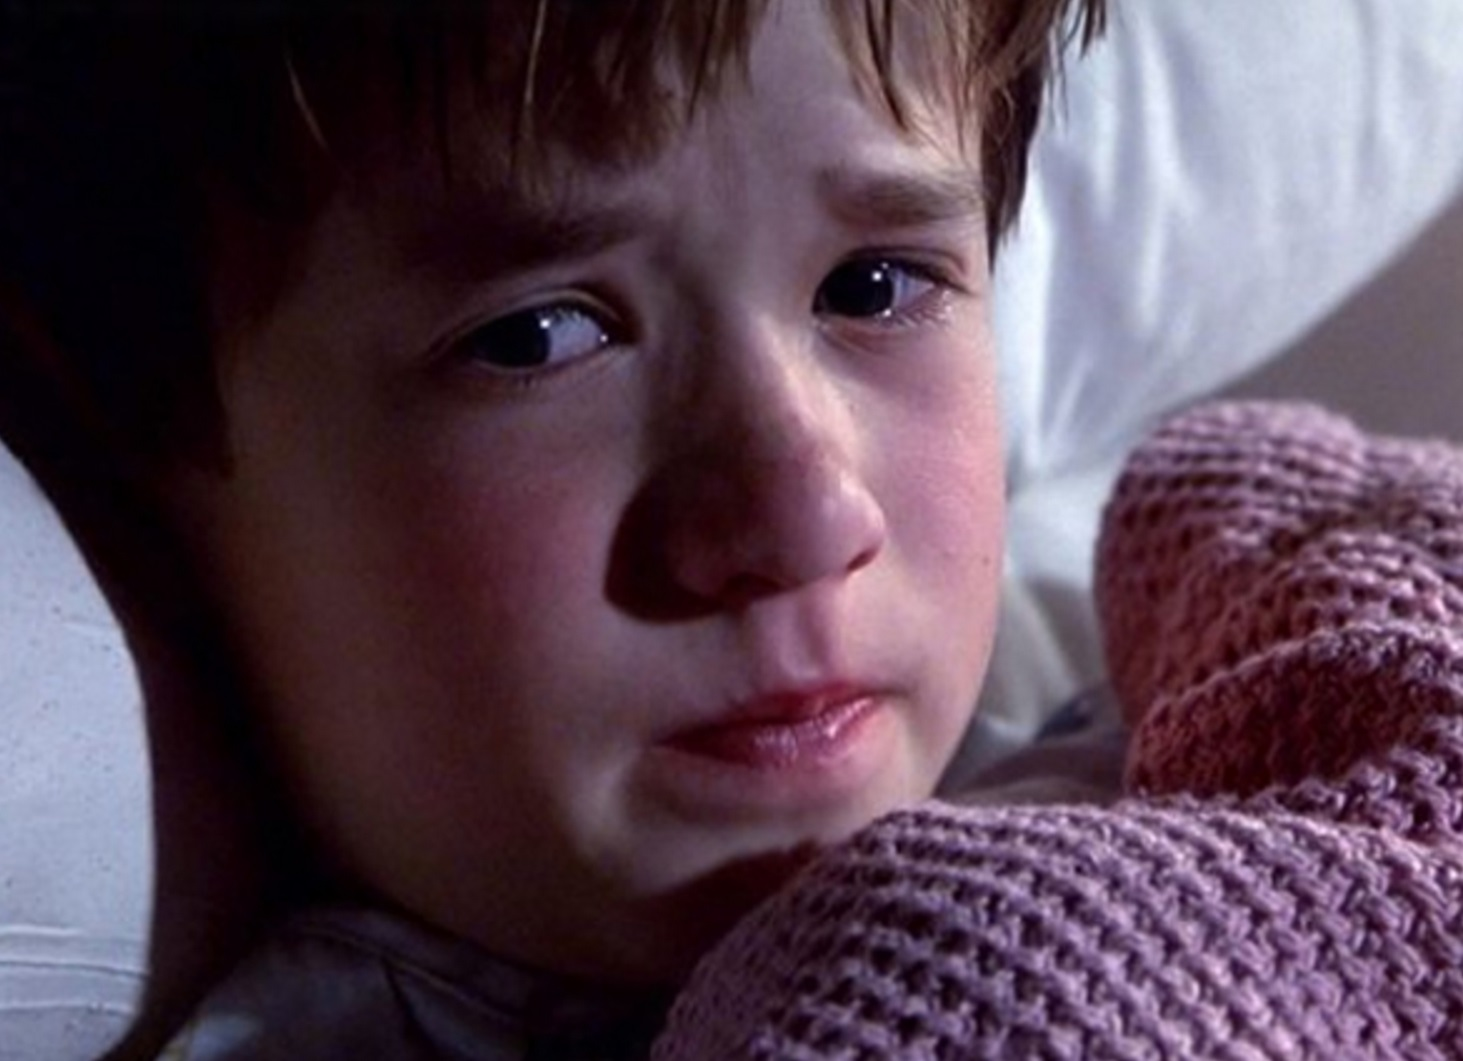
\includegraphics[width=10cm]{o-sexto-sentido}
            \centering
            \end{figure}
            Esse icônico filme da decada de 90 será uma das princípais inspirações para a lore do jogo, principalmente quanto ao seu plot twist de o protagonista da historia estar morto desde o princípio e ir recebendo pequenas dicas deste fato no decorrer do filme, e para o público desatento que não percebeu, no final tambem acontece essa revelação, porém de maneira mais explicita. \\
 

    \subsection{Descrição do projeto}%
Em um cup noodles de frutos do mar, o unico camarão desidratado do pacote, solitário e na escuridão, tenta escapar de sua prisão, para voltar ao mar em busca de seu amor.\\
Embarque nessa jornada cheia de perigos e plataformas, usando sua poderosa pinça para esmagar inimigos que ficarem entre seu você e o amor verdadeiro, e se não ousarem chegar basta bater suas pinças para criar um pulso de agua capaz de destruir qualquer um.\\
Nada pode parar um camarão determinado\\

   
\section{História/Lore}%
    \subsection{Vida}%
Nas aguas do litoral do Rio de Janeiro, vive uma pequena comunidade de camarões de estalo, dentre eles, um indivíduo nos interessa, Shu Rimp da Silva, esse camarão, apesar de pequeno, carrega em seu braço direito um poderosa pinça capaz de disparar projeteis de bolhas pela agua, carinhosamente apelidada de "38Tão".\\
Shu vive com sua família, esposa e filhos, uma vida tranquila e sem grandes surpresas, de certa forma até monotona, entretanto um acontecimento mudou tudo.
    \subsection{Morte}%
Um dia, caçadores de camarão invadiram a pequena comunidade, que mesmo com seus poderosos estalos foram incapazes de se defender, muitos camarões foram capturados neste dia, inclusive Shu. Esse grupo de camarões capturados tiveram o infortunio de serem destinados a fabrica de um produto singular, o CapNoodles de frutos do mar, um alimento feito com o tradicional macarrão instantâneo e varios produtos desidratados\\
Ao chegarem na fabrica os capturados foram separado uns dos outros, desidratados e colocados em uma unidade do produto, morrendo durante o processo, entretanto, um deles, com sua extrema força de vontade iria acordar.\\
    \subsection{Pós-vida}%
A partir desse ponto se passa a historia do jogo, nosso heroi Shu acorda de seu "sono", sem lembrar de parte do que aconteceu, mas com apenas um objetivo em mente, voltar para seu lar.\\
A primeira coisa a se fazer é libertar-se de sua prisão de papelão e plástico, e então, avançar incansavelmente em direção ao mar. Durante essa jornada Shu encontrara conhecidos que o ajudarão em seu objetivo, e desconhecidos tentando o impedir.\\
    \subsection{Tragédia}%
Após arduas batalhas, em um momento Shu finalmente chegará ao mar, entretanto não será um final feliz, pois finalmente descobrirá que durante todo esse tempo esteve morto, e que por isso não pode ficar junto de sua familia, seu principal objetivo
